\everymath{\displaystyle}
\documentclass{beamer}
% \documentclass[handout]{beamer}

%\usepackage[pdftex]{color,graphicx}
\usepackage{amsmath,amssymb,amsfonts}

\mode<presentation>
{
  % \usetheme{Darmstadt}
  % \usetheme[hideothersubsections]{Hannover}
  % \usetheme[hideothersubsections]{Goettingen}
  \usetheme[hideothersubsections, right]{Berkeley}

  \usecolortheme{seahorse}
  % \usecolortheme{dolphin}
  \usecolortheme{rose}
  % \usecolortheme{orchid}

  \useinnertheme[shadow]{rounded}

  % \setbeamercovered{transparent}
  \setbeamercovered{invisible}
  % or whatever (possibly just delete it)
}

\mode<handout>{
  \setbeamercolor{background canvas}{bg=black!5}
  \usepackage{pgfpages}
  \pgfpagesuselayout{4 on 1}[a4paper,border shrink=5mm, landscape]
}

\usepackage[brazilian]{babel}
% or whatever

% \usepackage[latin1]{inputenc}
\usepackage[utf8]{inputenc}
% or whatever

\usepackage{times}
%\usepackage[T1]{fontenc}
% Or whatever. Note that the encoding and the font should match. If T1
% does not look nice, try deleting the line with the fontenc.


\title%[] % (optional, use only with long paper titles)
{A distribuição Normal}

\subtitle
{Distribuição Normal, e IC da média} % (optional)

\author%[] % (optional, use only with lots of authors)
{Felipe Figueiredo}% \and S.~Another\inst{2}}
% - Use the \inst{?} command only if the authors have different
%   affiliation.

\institute[] % (optional, but mostly needed)
{
}
  % \inst{1}%
  % Department of Computer Science\\
  % University of Somewhere
  % \and
  % \inst{2}%
  % Department of Theoretical Philosophy\\
  % University of Elsewhere}
% - Use the \inst command only if there are several affiliations.
% - Keep it simple, no one is interested in your street address.

\date%[] % (optional)
{}

% \subject{Talks}
% This is only inserted into the PDF information catalog. Can be left
% out. 



% If you have a file called "university-logo-filename.xxx", where xxx
% is a graphic format that can be processed by latex or pdflatex,
% resp., then you can add a logo as follows:

\pgfdeclareimage[height=1.6cm]{university-logo}{../logo}
\logo{\pgfuseimage{university-logo}}



% Delete this, if you do not want the table of contents to pop up at
% the beginning of each subsection:
\AtBeginSubsection[]
%\AtBeginSection[]
{
  \begin{frame}<beamer>{Sumário}
    \tableofcontents[currentsection,currentsubsection]
  \end{frame}
}


% If you wish to uncover everything in a step-wise fashion, uncomment
% the following command: 

% \beamerdefaultoverlayspecification{<+->}

\usepackage[normalem]{ulem}

\begin{document}

\begin{frame}
  \titlepage
\end{frame}

\begin{frame}{Sumário}
  \tableofcontents
  % You might wish to add the option [pausesections]
\end{frame}


%% Template
% \section{}

% \subsection{}

% \begin{frame}{}
%   \begin{itemize}
%   \item 
%   \end{itemize}
% \end{frame}

% \begin{frame}
%   \begin{columns}
%     \begin{column}{5cm}
%     \end{column}
%     \begin{column}{5cm}
%     \end{column}
%   \end{columns}
% \end{frame}

% \begin{frame}{}
%   \includegraphics[height=0.4\textheight]{file1}
%   \includegraphics[height=0.4\textheight]{file2}
%   \includegraphics[height=0.4\textheight]{file3}
%   \begin{figure}
%     \caption{}
%   \end{figure}
% \end{frame}

% \begin{frame}{}
%   \begin{definition}
%   \end{definition}
%   \begin{example}
%   \end{example}
%   \begin{block}{Exercício}
%   \end{block}
% \end{frame}

% \section{Discussão da aula passada}

% \subsection{Discussão da aula passada}

\begin{frame}{\scriptsize Discussão da aula passada}
  \begin{block}{}
    Discussão da leitura obrigatória da aula passada
  \end{block}
\end{frame}

\section{A distribuição Normal}

\begin{frame}[label=oquee]{\scriptsize Pergunta central da aula}
  \begin{block}{}
    \Large\centering
    O que é o IC em torno da média?
  \end{block}
\end{frame}

\subsection{Distribuições de probabilidade}

\begin{frame}{\scriptsize Recapitulando}
  \begin{columns}
    \begin{column}{5cm}
      \begin{itemize}
        \scriptsize
      \item ({\tiny aula passada})
        \bigskip
      \item Pressão sanguínea (PS) de todos os 100 alunos de uma sala
        \medskip
      \item Visualização da média e variabilidade dos dados
      \end{itemize}
    \end{column}
    \begin{column}{5cm}
      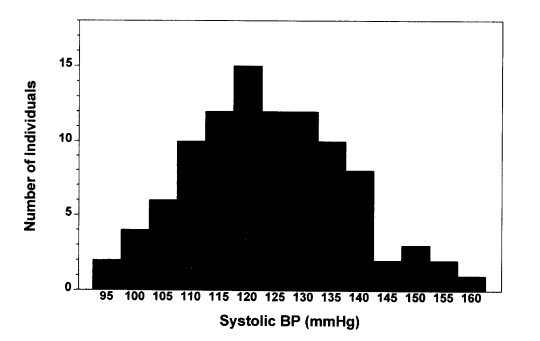
\includegraphics[width=\textwidth]{Cap3/histograma1}
    \end{column}
  \end{columns}
\end{frame}

\begin{frame}{\scriptsize Distribuições de probabilidade - Por que?}
  \begin{itemize}
    \footnotesize
  \item Distribuições teóricas = \alert{modelos} da realidade
  \item Aprender com os modelos $\Rightarrow$ ferramenta
  \end{itemize}
  \begin{block}{Na vida real}
    \footnotesize
    Distribuição ``próxima'' de um modelo $\Rightarrow$ metodologia
  \end{block}
\end{frame}

\begin{frame}[label=exemplo5.1]{\scriptsize Distribuições de dados ``reais''}
  \begin{exampleblock}{Exemplo 5.1}
    \scriptsize
    No exemplo, a PS dos 100 alunos (a turma inteira) foi visualizada em um histograma.

    \bigskip
    Calculando a média, encontramos $\bar{x}$ = 123,4 mmHg.

    Calculando o DP, encontramos $s$ = 14,0 mmHg.
  \end{exampleblock}
  \begin{block}{Pense...}
    \footnotesize
    \begin{itemize}
      \scriptsize
    \item Se a população for a turma, sabemos a média e o DP {\bf com certeza}
    \item Se a turma é uma amostra de uma população maior, como podemos {\em inferir} os parâmetros da população (digamos, com 95\% de confiança)?
    \end{itemize}
  \end{block}
\end{frame}

\begin{frame}{\scriptsize Distribuições de dados ``reais''}
  \begin{columns}
    \begin{column}{5cm}
      \begin{exampleblock}{Exemplo 5.1}
        \footnotesize
        \begin{itemize}
          \scriptsize
        \item $\bar{x}$ = 123,4 mmHg
        \item $s$ = 14,0 mmHg
        \end{itemize}
      \end{exampleblock}
      \begin{block}{}
        \footnotesize
        \begin{itemize}
          \scriptsize
        \item Você  {\em vê} a média?
        \item Você  {\em vê} o DP?
        \end{itemize}
      \end{block}
    \end{column}
    \begin{column}{5cm}
      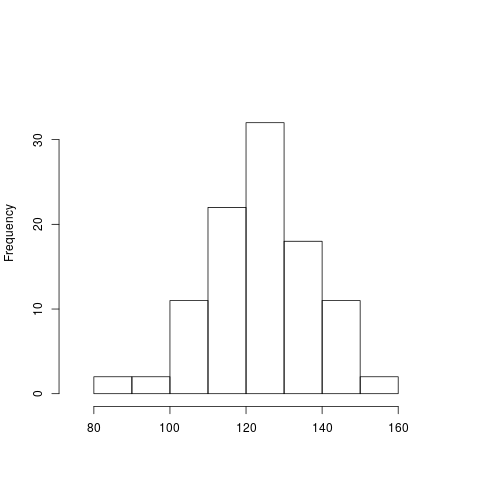
\includegraphics[width=\textwidth]{Cap4/normal1}
    \end{column}
  \end{columns}
\end{frame}

\begin{frame}{\scriptsize Observações importantes}
  \begin{columns}
    \begin{column}{5cm}
      \begin{itemize}
        \tiny
      \item Muitas medições próximas da média
        \medskip
      \item Poucas medições de PS muito baixas
        \medskip
      \item Poucas medições de PS muito altas
        \medskip
      \item Aprox. simétrica em torno da média
      \end{itemize}
    \end{column}
    \begin{column}{5cm}
      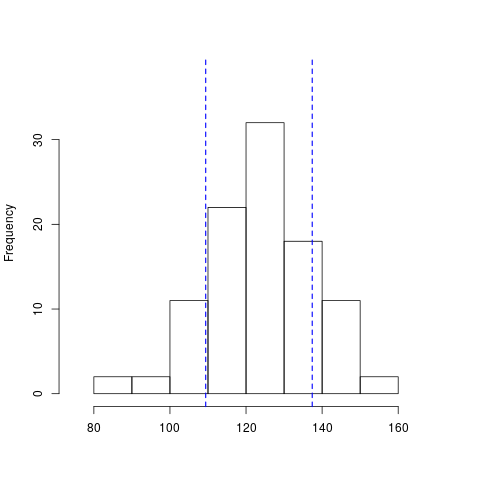
\includegraphics[width=\textwidth]{Cap4/normal3}
    \end{column}
  \end{columns}
\end{frame}

\subsection{A distribuição Normal}


\begin{frame}{\scriptsize Distribuição Normal}
  \begin{center}
    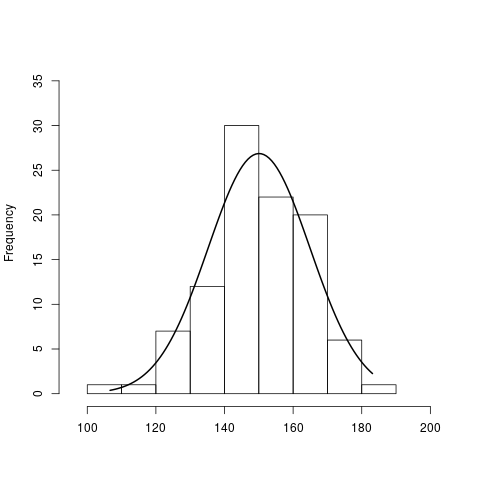
\includegraphics[height=\textheight]{Cap4/normal2}
  \end{center}
\end{frame}

\begin{frame}{\scriptsize Distribuição Normal, com DP}
  \begin{center}
    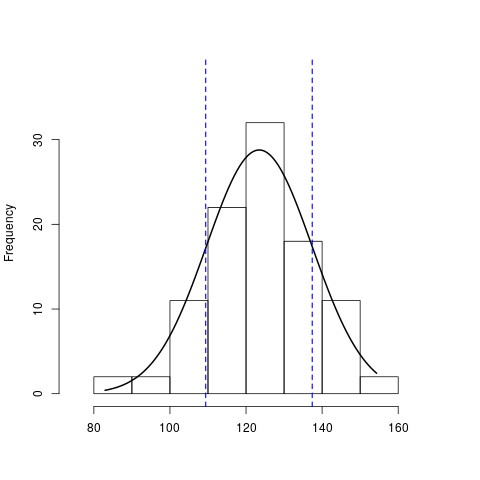
\includegraphics[height=\textheight]{Cap4/normal4}
  \end{center}
\end{frame}

\begin{frame}{\scriptsize E esta?}
  \begin{columns}
    \begin{column}{5cm}
      \begin{itemize}
        \tiny
      \item Muitas medições próximas da média?
        \medskip
      \item Poucas medições de PS muito baixas?
        \medskip
      \item Poucas medições de PS muito altas?
        \medskip
      \item Aprox. simétrica em torno da média?
      \end{itemize}
    \end{column}
    \begin{column}{5cm}
      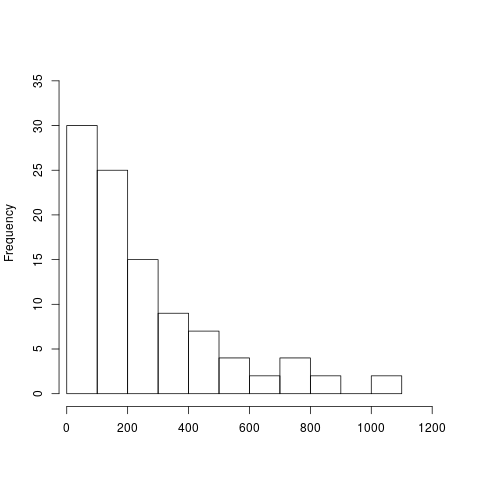
\includegraphics[width=\textwidth]{Cap4/lognormal}
    \end{column}
  \end{columns}
\end{frame}

\begin{frame}{\scriptsize E esta?}
  \begin{columns}
    \begin{column}{5cm}
      \begin{itemize}
        \tiny
      \item Muitas medições próximas da média?
        \medskip
      \item Poucas medições de PS muito baixas?
        \medskip
      \item Poucas medições de PS muito altas?
        \medskip
      \item Aprox. simétrica em torno da média?
      \end{itemize}
    \end{column}
    \begin{column}{5cm}
      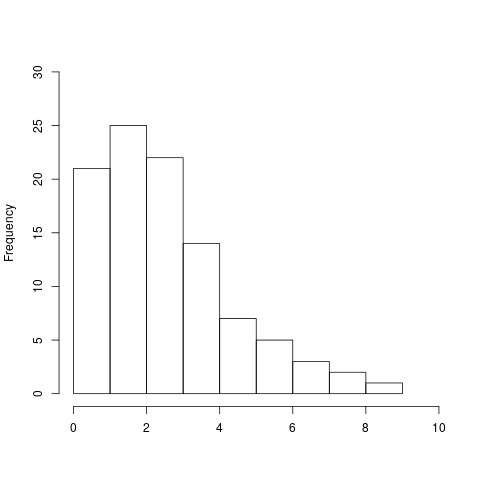
\includegraphics[width=\textwidth]{Cap4/poisson}
    \end{column}
  \end{columns}
\end{frame}

\begin{frame}{\scriptsize E esta?}
  \begin{columns}
    \begin{column}{5cm}
      \begin{itemize}
        \tiny
      \item Muitas medições próximas da média?
        \medskip
      \item Poucas medições de PS muito baixas?
        \medskip
      \item Poucas medições de PS muito altas?
        \medskip
      \item Aprox. simétrica em torno da média?
      \end{itemize}
    \end{column}
    \begin{column}{5cm}
      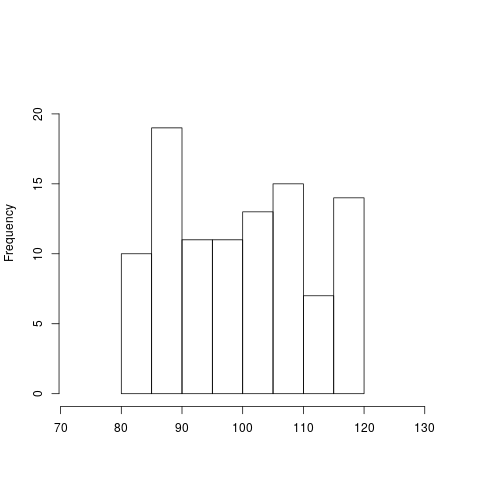
\includegraphics[width=\textwidth]{Cap4/uniforme}
    \end{column}
  \end{columns}
\end{frame}

\subsection{Inferências}

\begin{frame}{\scriptsize A regra empírica}
  \begin{itemize}
    \footnotesize
  \item ({\tiny aula passada})
        \bigskip
  \item ``mais da metade'' dos dados estão a 1 DP da média
        \bigskip
  \item ``quase todos'' os dados estão a 2 DPs da média
  \end{itemize}
\end{frame}

\begin{frame}{\scriptsize A regra empírica}
  \begin{columns}
    \begin{column}{5cm}
      \begin{itemize}
        \footnotesize
      \item 68\% a até 1 DP da média
        \medskip
      \item 95\% a até 2 DP da média
        \medskip
      \item 99,7\% a até 3 DP da média
      \end{itemize}
    \end{column}
    \begin{column}{5cm}
      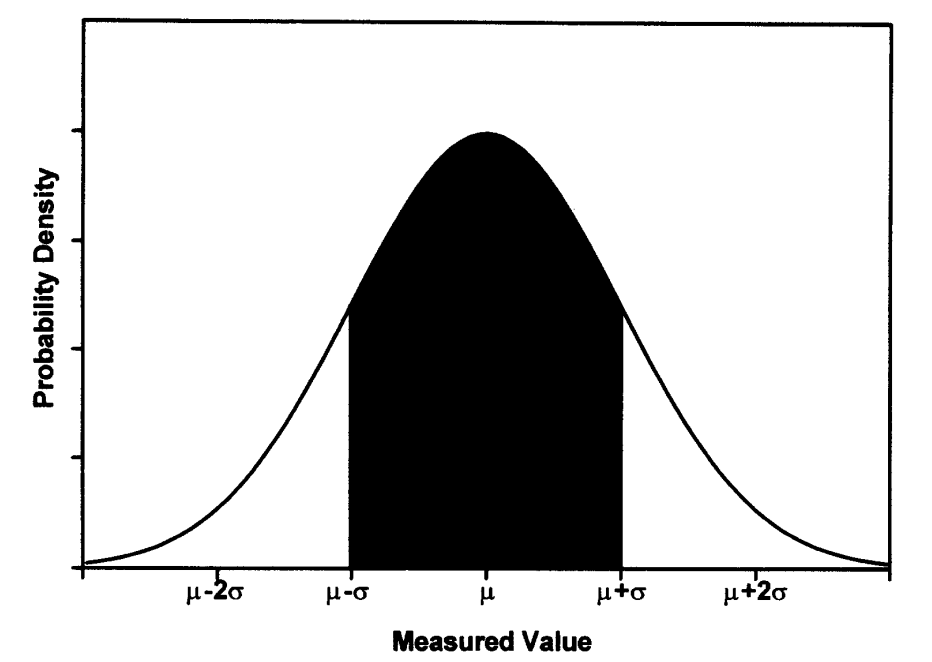
\includegraphics[width=\textwidth]{Cap4/empirica}
    \end{column}
  \end{columns}
\end{frame}

\begin{frame}{\scriptsize Atenção}
  \begin{block}{}
    \begin{center}
      \Large
      A regra empírica assume que...

      \bigskip
      ... os dados são normalmente distribuídos.
    \end{center}
  \end{block}
\end{frame}

\section{IC da média}

\subsection{Interpretação}

\begin{frame}{\scriptsize Exemplos}
  \begin{center}
    Vamos recapitular o exemplo 5.1, antes de introduzir outro.
  \end{center}
\end{frame}

\againframe{exemplo5.1}

\begin{frame}{\scriptsize Distribuições de dados ``reais''}
  \begin{exampleblock}{Exemplo 5.2}
    \scriptsize
    Das 100 medições de PS, você amostrou aleatoriamente 5 medições.

    Valores aproximados: 120, 80, 90, 110 e 95 mmHg.

    \bigskip
    Calculando a média, encontramos $\bar{x}$ = 99,0 mmHg.

    Calculando o DP, encontramos $s$ = 15,97 mmHg.
  \end{exampleblock}
  \begin{block}{Pense...}
    \footnotesize
    \begin{itemize}
      \scriptsize
    \item Se a população for a turma, podemos estimar a média e o DP da turma com os valores desta amostra?
    \item Se a turma é uma amostra de uma população maior, esta estimativa nos dá ``mais confiança'' sobre a população, ou menos?
    \end{itemize}
  \end{block}
\end{frame}

\begin{frame}{\scriptsize IC da média}
  \begin{exampleblock}{ICs dos exemplos}
    \footnotesize
    \begin{itemize}
      \footnotesize
    \item IC do exemplo 5.1: 120,6 até 126,2 mmHg
        \medskip
    \item IC do exemplo 5.2: 79,2 até 118,8 mmHg
    \end{itemize}
  \end{exampleblock}
  \begin{block}{Relembre...}<2->
    \footnotesize
    O que significa o IC?
  \end{block}
  \begin{block}{Pense...}
    \footnotesize
    Observe os tamanhos dos ICs.
  \end{block}
\end{frame}

\subsection{Premissas}

\begin{frame}{\scriptsize Premissas}
  \scriptsize
  Assumimos que estas coisas são verdadeiras para calcular/interpretar um IC
  \bigskip
  \bigskip
  \begin{itemize}
    \scriptsize
  \item A amostra foi selecionada aleatoriamente da população (sem reposição)
  \medskip
  \item A população é Normal (Gaussiana)
  \medskip
  \item Os indivíduos são independentes, uns dos outros
  \end{itemize}
\end{frame}

\subsection{O Erro Padrão}

\begin{frame}{\scriptsize Teorema do Limite Central}
  Vídeo
\end{frame}

\begin{frame}{\scriptsize Variabilidade x Erro Padrão}
  \begin{block}{Variabilidade}
    \footnotesize
    A variabilidade nos informa sobre a dispersão da amostra/população.
  \end{block}
  \begin{block}{O erro padrão}
    \footnotesize
    O Erro Padrão nos informa quão boa é nossa \alert{estimativa} da média.
  \end{block}
\end{frame}

\begin{frame}{\scriptsize O Erro Padrão - definição}
  \begin{displaymath}
    SEM = \frac{s}{\sqrt{n}}
  \end{displaymath}
  \bigskip
  \begin{itemize}
    \scriptsize
  \item SEM = Erro Padrão da Média ({\tiny em inglês})
    \medskip
  \item Conforme $n$ aumenta $\Rightarrow$ SEM diminui
    \medskip
  \item Conforme $n$ aumenta $\Rightarrow$ $\bar{x}$ ``próximo'' de $\mu$
  \end{itemize}
  \bigskip
  \begin{block}{Lembrete}
    \tiny
    \begin{itemize}
    \footnotesize
    \item $\bar{x}$ -- média da amostra (resultado/possível)
    \item $\mu$ -- média da população (objetivo/inferência)
    \end{itemize}
  \end{block}
\end{frame}

\begin{frame}{\scriptsize O Erro Padrão - Interpretação}
  \begin{block}{Interpretação}
    \footnotesize
    Quando queremos {\bf inferir} a média da população a partir de uma amostra, qual é a incerteza associada a esta estimativa?
  \end{block}
  \begin{block}{Pense...}<2->
    \footnotesize
    E o desvio-padrão $s$?
  \end{block}
\end{frame}

\begin{frame}{\scriptsize O Erro Padrão}
  \begin{displaymath}
    IC: \bar{x} \pm t^{*} \times SEM
  \end{displaymath}
  \begin{itemize}
    \footnotesize
  \item $\bar{x}$ = média
  \item Para amostras {\bf grandes}, $t^{*} \approx$ 2.
  \end{itemize}
\end{frame}

\begin{frame}{\scriptsize O Erro Padrão - IC da média}
  \begin{displaymath}
    IC: \bar{x} \pm t^{*} \times SEM
  \end{displaymath}
  \begin{block}{Perguntas}
    \begin{enumerate}
      \footnotesize
    \item<1-> Se $s$ aumenta, o SEM aumenta ou diminui?
    \item<2-> Se $s$ aumenta, o IC aumenta ou diminui?
    \item<3-> Se $t^{*}$ aumenta, o IC aumenta ou diminui?
    \end{enumerate}
  \end{block}
\end{frame}

\begin{frame}{\scriptsize O Erro Padrão}
  \begin{displaymath}
    IC: \bar{x} \pm 2\footnote{$t^{*} \approx$ 2} \times SEM
  \end{displaymath}
  \begin{exampleblock}{Exemplo 5.1}
    \footnotesize
    \begin{itemize}
      \tiny
    \item $s$ = 14,0 e N = 100
    \item $SEM = \frac{14}{\sqrt{100}} = 1.4$
    \item IC =  $123.4 \pm 2 \times 1.4$
    \item IC =  $123.4 \pm 2.8$
      \bigskip
      \scriptsize
    \item IC $\approx$ [120.6, 126.2]
    \end{itemize}
  \end{exampleblock}
\end{frame}

\begin{frame}{\scriptsize Pense...}
  \begin{exampleblock}{ICs dos exemplos}
    \footnotesize
    \begin{itemize}
      \footnotesize
    \item {\bf Ex. 5.1:} $\bar{x}$ = 123,4 e $s$ = 14,0 mmHg ($N=100$)
    \item {\bf Ex. 5.2:} $\bar{x}$ = 99,0 e $s$ = 15,97 mmHg ($N=5$)
    \end{itemize}
  \end{exampleblock}
    \bigskip
  \begin{block}{Podemos reproduzir o mesmo método do 5.1 no 5.2?}
    \footnotesize
  \begin{itemize}
    \footnotesize
  \item SEM do exemplo 5.1 = 1,4
  \item SEM do exemplo 5.2 = 6,3?
  \end{itemize}
  \end{block}
\end{frame}

\begin{frame}{\scriptsize }
    \begin{block}{Podemos reproduzir o mesmo método do 5.1 no 5.2?}
    \footnotesize
  \begin{itemize}
    \footnotesize
  \item SEM do exemplo 5.1 = 1,4
  \item SEM do exemplo 5.2 = 6,3?
  \end{itemize}
  \end{block}
  \bigskip
  \begin{block}{Resposta}
    \footnotesize
    Não! Pois N=5 não é grande!

    \medskip
    Isso faz com que o SEM do exemplo 5.2 seja muito maior (como vimos).
  \end{block}
  \begin{exampleblock}{Lembrete -- ICs dos exemplos}
    \footnotesize
    \begin{itemize}
      \scriptsize
    \item O IC do exemplo 5.1: 120,6 -- 126,2 mmHg
    \item O IC do exemplo 5.2: 79,2 -- 118,8 mmHg
    \end{itemize}
  \end{exampleblock}
\end{frame}

\begin{frame}{\scriptsize }
  \begin{exampleblock}{Lembrete -- ICs dos exemplos}
    \footnotesize
    \begin{itemize}
      \footnotesize
    \item O IC do exemplo 5.1: 120,6 -- 126,2 mmHg
    \item O IC do exemplo 5.2: \alert{79,2 -- 118,8 mmHg}
    \end{itemize}
  \end{exampleblock}
  \begin{block}{No caso do exemplo 5.2}
    \footnotesize
    \begin{itemize}
      \footnotesize
    \item $\bar{x} = 99$ mmHg
    \item O SEM proposto no slide anterior é $\approx$ 6 mmHg
    \item A margem de erro seria {\bf 2} $\times $ 6 $\approx$ 12 mmHg
    \end{itemize}
      $\Rightarrow$ O IC proposto seria \alert{87 -- 111 mmHg}
  \end{block}
  \begin{block}{Pense...}
    \footnotesize
    Qual parece ser a margem de erro {\em real} do IC acima?
  \end{block}
\end{frame}

\begin{frame}{\scriptsize }
  \begin{exampleblock}{Lembrete -- ICs dos exemplos}
    \footnotesize
    \begin{itemize}
      \footnotesize
    \item O IC do exemplo 5.1: 120,6 -- 126,2 mmHg
    \item O IC do exemplo 5.2: \alert{79,2 -- 118,8 mmHg}
    \end{itemize}
  \end{exampleblock}
  \begin{block}{No caso do exemplo 5.2}
    \footnotesize
    \begin{itemize}
      \footnotesize
    \item O SEM veio da ``fórmula''
    \item Ambos SEM (5.1 e 5.2) estão corretos
    \item O IC proposto seria \alert{87 -- 111 mmHg}
    \item $t^{*} \approx$ 2 -- erro no 5.2
    \end{itemize}
  \end{block}
  \begin{block}{Pense...}
    \footnotesize
    Qual é a sua conclusão sobre esse $t^{*}$ misterioso?
  \end{block}
\end{frame}

\begin{frame}
  \begin{center}
    \LARGE
    Quiz!
  \end{center}
\end{frame}

\begin{frame}{\scriptsize Quiz}
  \begin{block}{Pergunta}
    \footnotesize
    O erro padrão, assim como o desvio padrão, é uma medida descritiva de dispersão:

    \bigskip
    \begin{enumerate}
      \scriptsize
    \item Verdadeiro
    \item \alert<2>{Falso}
      \invisible{
    \item 1
    \item 1
      }
    \end{enumerate}
  \end{block}
\end{frame}

\begin{frame}{\scriptsize Quiz}
  \begin{block}{Pergunta}
    \footnotesize
    São necessários para p cálculo do IC em torno da média:

    \bigskip
    \begin{enumerate}
      \scriptsize
    \item \alert<2>{Desvio padrão (s)}
    \item \alert<2>{Observações independentes}
    \item \alert<2>{Erro padrão (SEM)}
    \item \alert<2>{N}
    \end{enumerate}
  \end{block}
\end{frame}

\begin{frame}{\scriptsize Quiz}
  \begin{block}{Pergunta}
    \footnotesize
    Existem infinitas distribuições Normais.

    \bigskip
    \begin{enumerate}
      \scriptsize
    \item \alert<2>{Verdadeiro}
    \item Falso
      \invisible{
    \item 1
    \item 1
      }
    \end{enumerate}
  \end{block}
\end{frame}

\againframe{oquee}

\section{Aprofundamento}

\subsection{Aprofundamento}

\begin{frame}{\scriptsize Aprofundamento}
  \begin{block}{Leitura obrigatória}
    \begin{itemize}
      \footnotesize
    \item Capítulo 4. Pular a seção {\bf Intervalo de Predição}.
    \item Capítulo 5. Pular as seções:
      \begin{itemize}
        \scriptsize
      \item Calculando o IC da média
      \item A distribuição {\em t} ({\tiny será abordado na próxima aula})
      \end{itemize}
    \end{itemize}
  \end{block}
  \begin{block}{Leitura recomendada}
    \scriptsize
    Capítulo 4. seção {\bf Intervalo de Predição}.
  \end{block}
\end{frame}

\end{document}
